% !TEX encoding = UTF-8
% !TEX TS-program = pdflatex
% !TEX root = ../Tesi.tex
% !TEX spellcheck = it-IT

%************************************************
\chapter{Introduzione allo logica dello spazio}
\label{cap:spazio}
%************************************************

\begin{flushright}{\slshape
  …sì, per cui una chiesa barocca ha sotto di sé, \\
  accessibile, una chiesa romanica, \\
  sotto la chiesa romanica una basilica paleocristiana, \\
  poi si scende ancora e c’è il mitreo romano… \\
  Questa è Roma. \\
  Però, invece, apparentemente Roma è appunto atemporale, \\
  sembra non offrire nulla; \\
  e gli accessi sono segreti, alla vera realtà di Roma. \\
  Quindi corrisponde assai bene allo stadio opaco dell’infanzia e dell’adolescenza, \\
  quando si è in preda a questa cosa strana che è il voler scrivere…} \\ \medskip
    --- G. Agamben
\end{flushright}


%\begin{figure}
%\centering
%\subfloat[Tetraedro inscritto in un cubo]
%{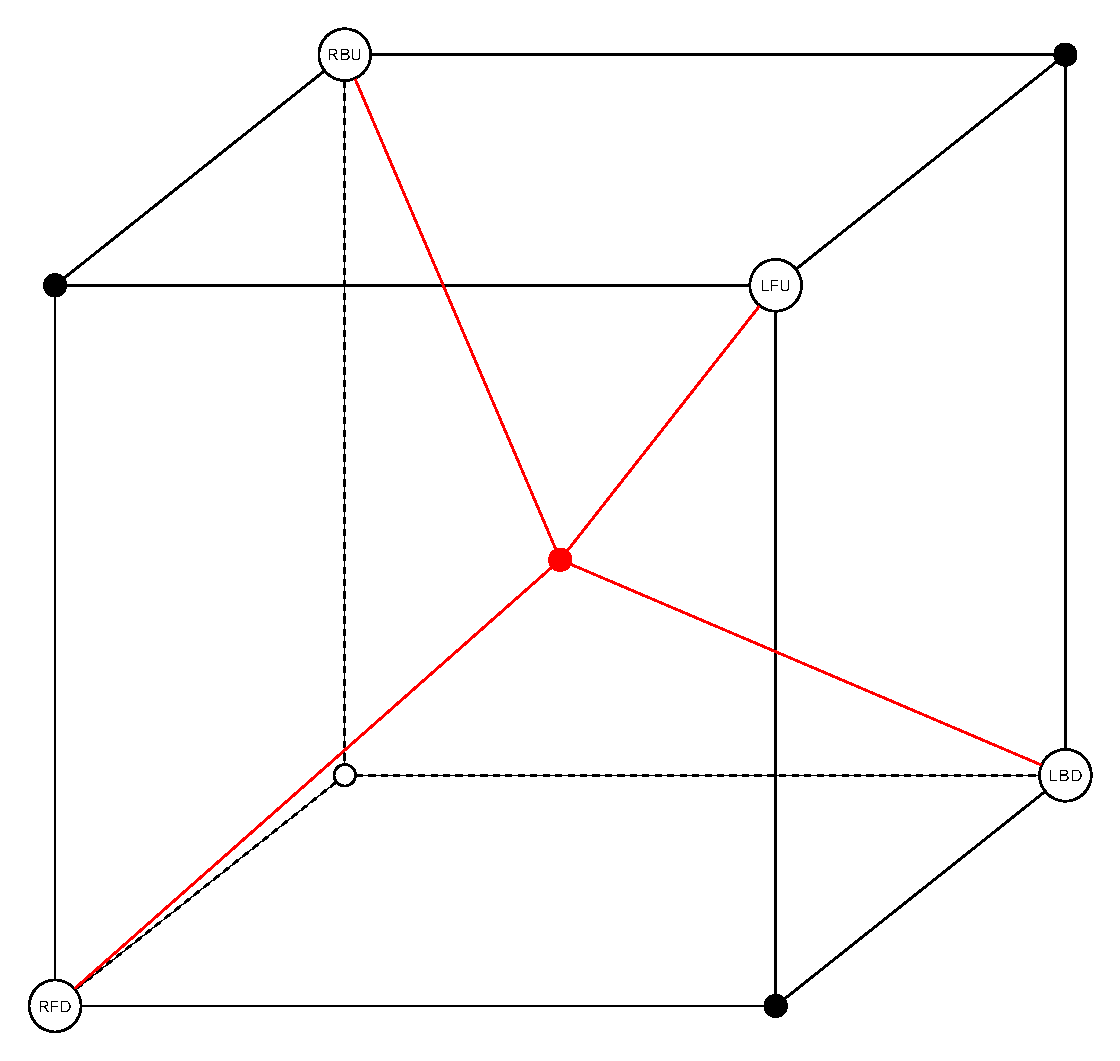
\includegraphics[width=.45\columnwidth]{tetrarec-cube}} \quad
%\subfloat[Spazio Tetraedrico]
%{\label{fig:tetracube}%
%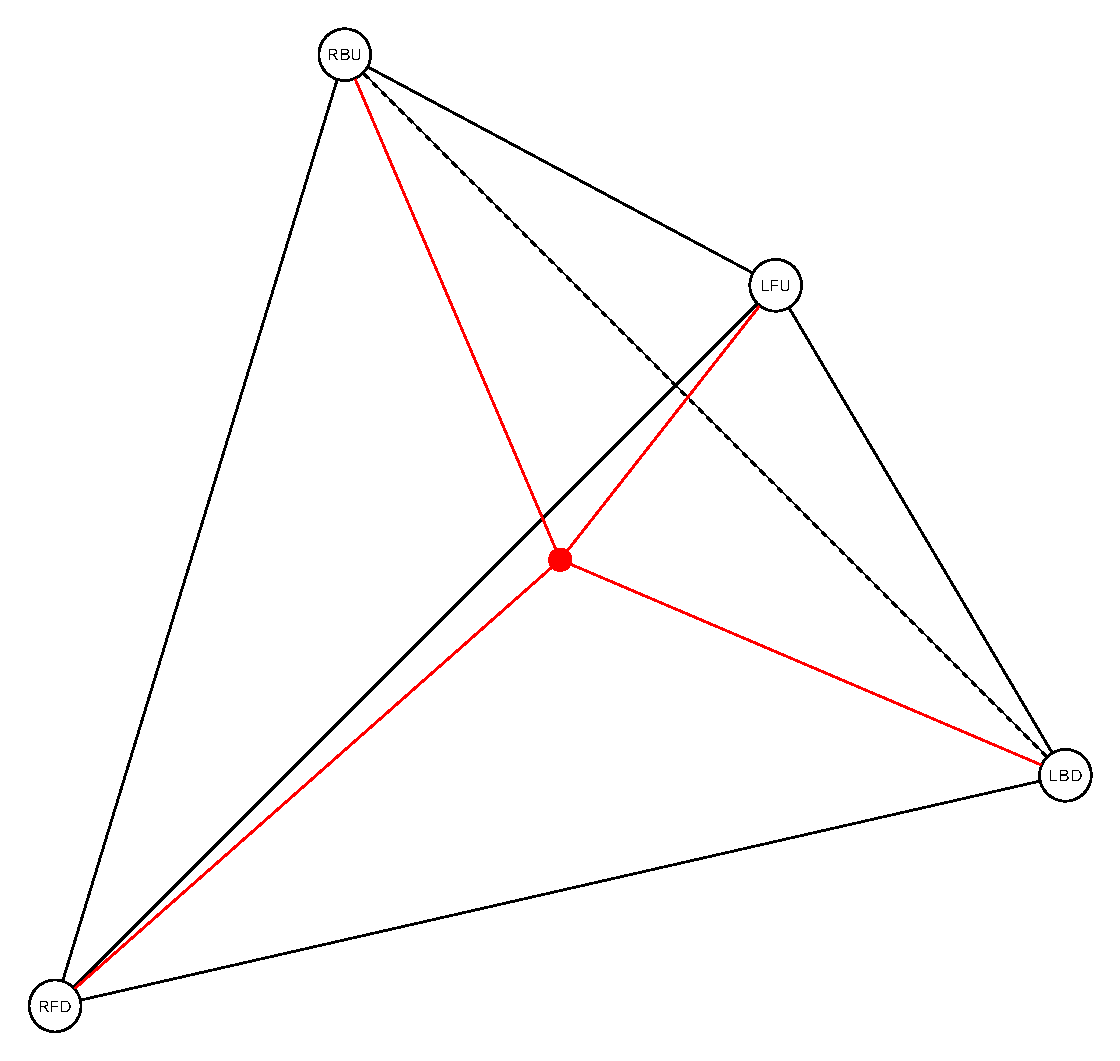
\includegraphics[width=.45\columnwidth]{tetrarec-tetrahedron}} \\
%\caption[Spazio Tetraedrico]{Spazio Tetraedrico}
%\label{fig:tetratetra}
%\end{figure}


%\begin{figure}
%\centering
%{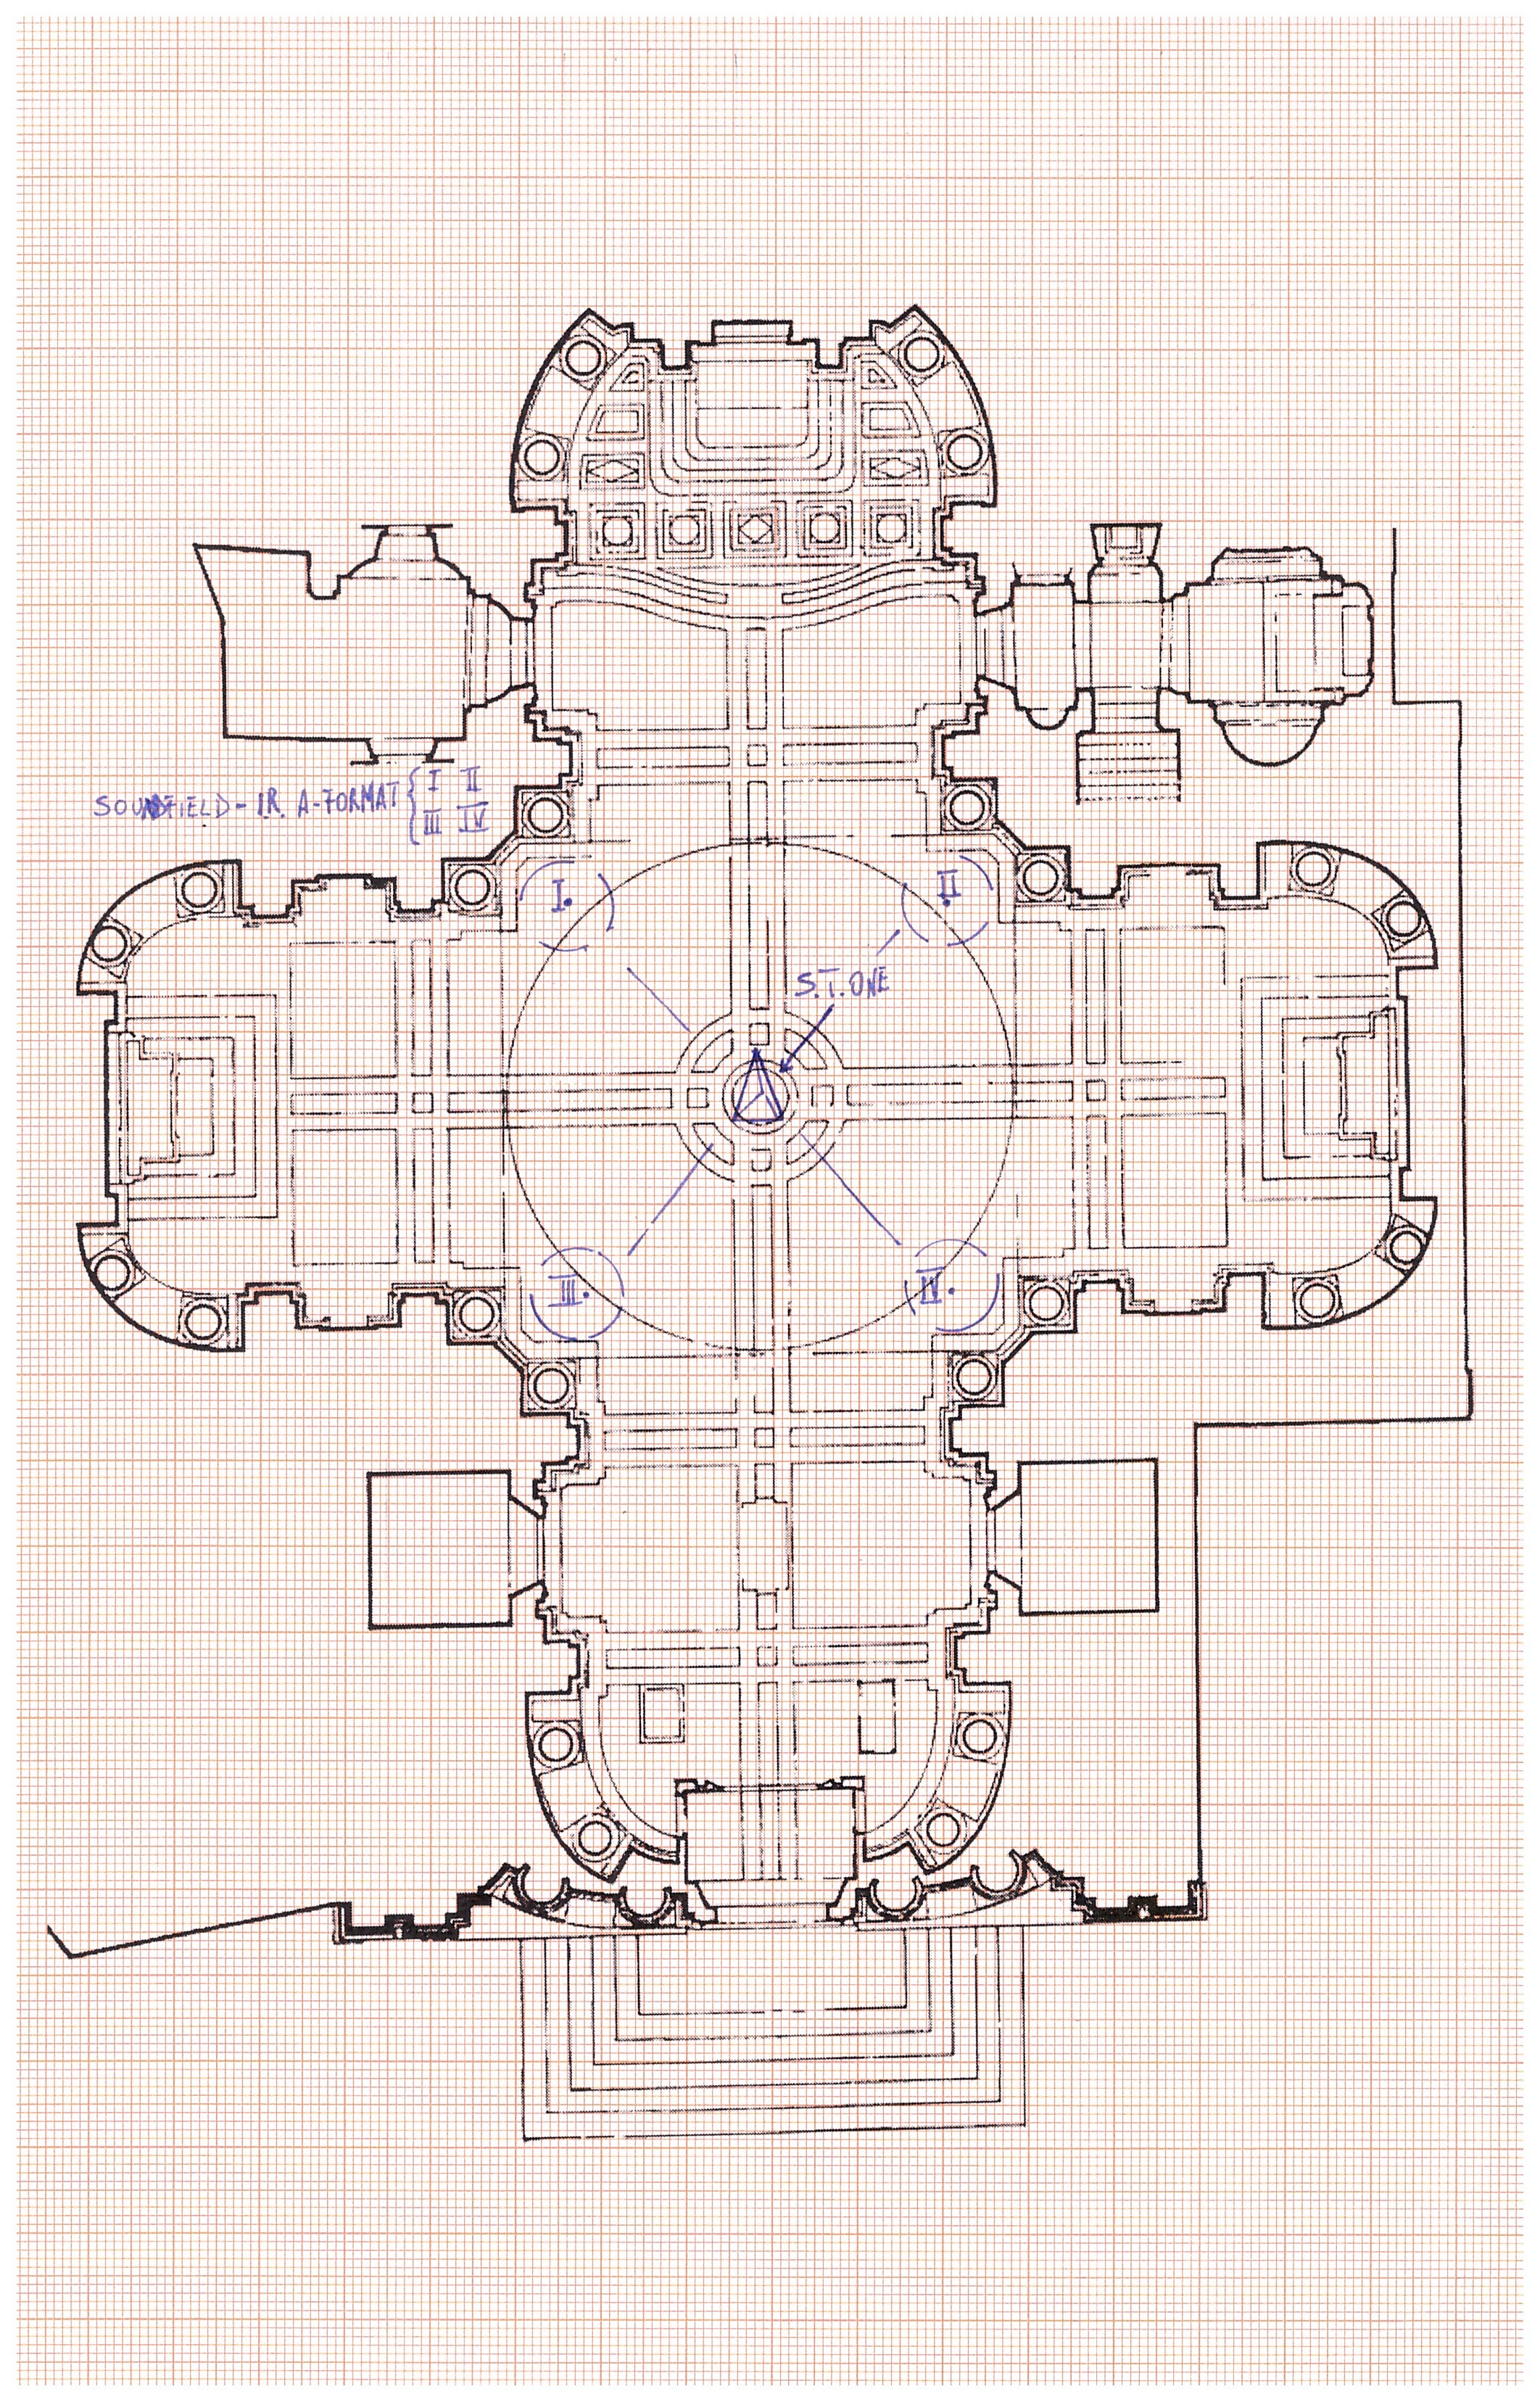
\includegraphics[width=.95\columnwidth]{Pianta_chiesa}}
%\caption[Pianta S. Luca]{Pianta S. Luca}
%\label{fig:tetratetra}
%\end{figure}

discorso riverbero non come elaborazione dell'amplificazione ma come costruzione delle
riflesioni ambientali. Le distanze hai 4 stone identisci cosi da dislocare gli altoparlanti
facilmente. Posto simmetrico posto. Filmarmonica in


%\begin{equation}
%\int_a^{a+T}f(x)\,dx= \int_0^T f(x)\,dx 
%\qquad
%\oint f(z)\,dz=2\pi i
%\end{equation}